\documentclass[../main.tex]{subfiles}
\graphicspath{{\subfix{../images/}}}
\begin{document}

\subsection{Transfer Learning}

The transfer learning technique uses a pre-trained model that classifies the images in one dataset and applies the outputs of that model to inform a different model of a different purpose. This is beneficial as the classes of the previous model can reveal patterns in the images that share properties with the 3 fruit. This means at least 1 additional layer needs to be added to map the outputs to the 3 classes of fruit.

To test this method, 2 pre-trained models will be used which are AlexNet and ResNet18. Both models were used on the ImageNet dataset. 

\begin{figure}[h!]
  \centering
  \begin{subfigure}[b]{0.35\linewidth}
    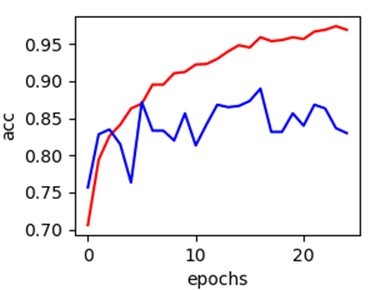
\includegraphics[width=\linewidth]{alexnet.png}
    \caption{Performance for AlexNet Transfer Learning}
  \end{subfigure}
  \begin{subfigure}[b]{0.35\linewidth}
    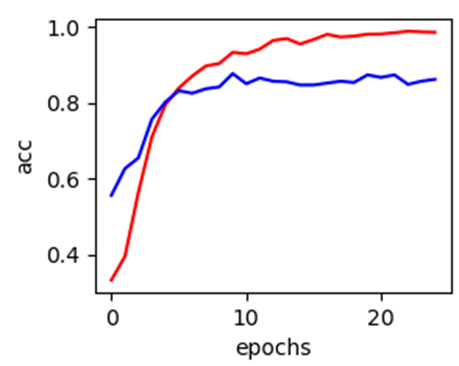
\includegraphics[width=\linewidth]{resnet18.png}
    \caption{Performance for ResNet18 Transfer Learning}
  \end{subfigure}
  \label{fig:Pre-Trained-Performance}
\end{figure}

It can be observed that both models reached a final accuracy of above 80\% within the first 10 epochs. This accuracy is better than the accuracy that was given by the model created. This suggest that the models have learnt patterns from the ImageNet dataset that can also be applied to this dataset of fruit. We see however that the accuracy of the AlexNet model is fluctuates unlike the ResNet18 which remained smooth. It is predicted if AlexNet could be trained for more epochs then it would converge to an accuracy around 85\% for the validation set. 

It can also be observed that the training set accuracy for both models are close to 100\%. This suggest that the model will become overfit if left continued to train which will decrease the accuracy of the validation set. This means that more layers after the initial pre-trained model is needed to improve the model. 

\end{document}